%\vspace{-0.07in}
\section{The General Case with Multiple Coflows}
%\vspace{-0.05in}
\label{sec:alg4}


Coflow scheduling under the general case introduces new challenges.
%The scheudling for the general case where multiple Coflows compete for network resources,
%Multiple coflows brings more challenges coflows favor different topologies,
Specially, since different coflows may favor different circuit configurations, the optimal solution (which minimizes the average CCT) should be a sequence of schedules, where each schedule is characterized by a different circuit configuration, routing, rate allocation and duration.
Compared to the case of coflow scheduling in packet switched networks (which is strongly NP-hard already \cite{varys}), the complexity of colfow scheduling in optical networks grows exponentially as we need to perform a joint scheduling of circuit configuration, routing/rate allocation, and coflow prioritization.

%Furthermore, the decisions for circuit configuration, permutation and rate/routing are tightly coupled and thus the complexity increases exponentially.
%an efficient decoupling of the

The key to perform efficient scheduling with reasonable complexity is to find a good way to decouple the problem. To this end,
we break the scheduling problem into three successive steps -- each determines the circuit configuration, permutation and rate/routing respectively.
And each step is further transformed into the single coflow scheduling problems (\ie, Problem \ref{problem:1}-\ref{problem:3}) formulated in Section \ref{sec:alg}. Similar to prior work on coflow scheduling \cite{varys,aalo,coda}, we coordinate coflow information to the central controller at $\sim$100$ms$ intervals, and run the inter-coflow scheduling framework (Figure \ref{fig:4}) at the beginning of every scheduling interval.  We briefly go through each step as follows.


%As we show in Figure \ref{fig:4}, such schedule is made at the beginning of every scheduling interval\footnote{Similar to prior work on coflow scheduling, we coordinate coflow information to the central controller at $\sim$100$ms$ intervals, and scheduling is done at the same pace.}. We briefly go through each step as follows.

\parab{Step 1: Circuit Configuration:}
Determine an appropriate circuit configuration for the current time slot is non-trivial.
One intuitive idea is to calculate a circuit that best serves the aggregated demand of \emph{all} current coflows. However, this is not necessarily a good idea, because the circuit can be reconfigured in the following timeslots. Since different coflows may favor different configurations, it is probably more efficient if we first configure the circuit to best serve the small coflows, and then reconfigure for the large coflows after the small coflows finish. As a result, there is no need to consider coflows which will be scheduled after a long time in the \emph{current} circuit configuration.
Another extreme is to always greedily optimize for the coflow with the highest priority. However doing so introduces too many reconfigurations, which also greatly enlarges the average CCT.
% (especially when the CCT is small compared to the reconfiguration cost).

\begin{figure}[t]
  \centering
  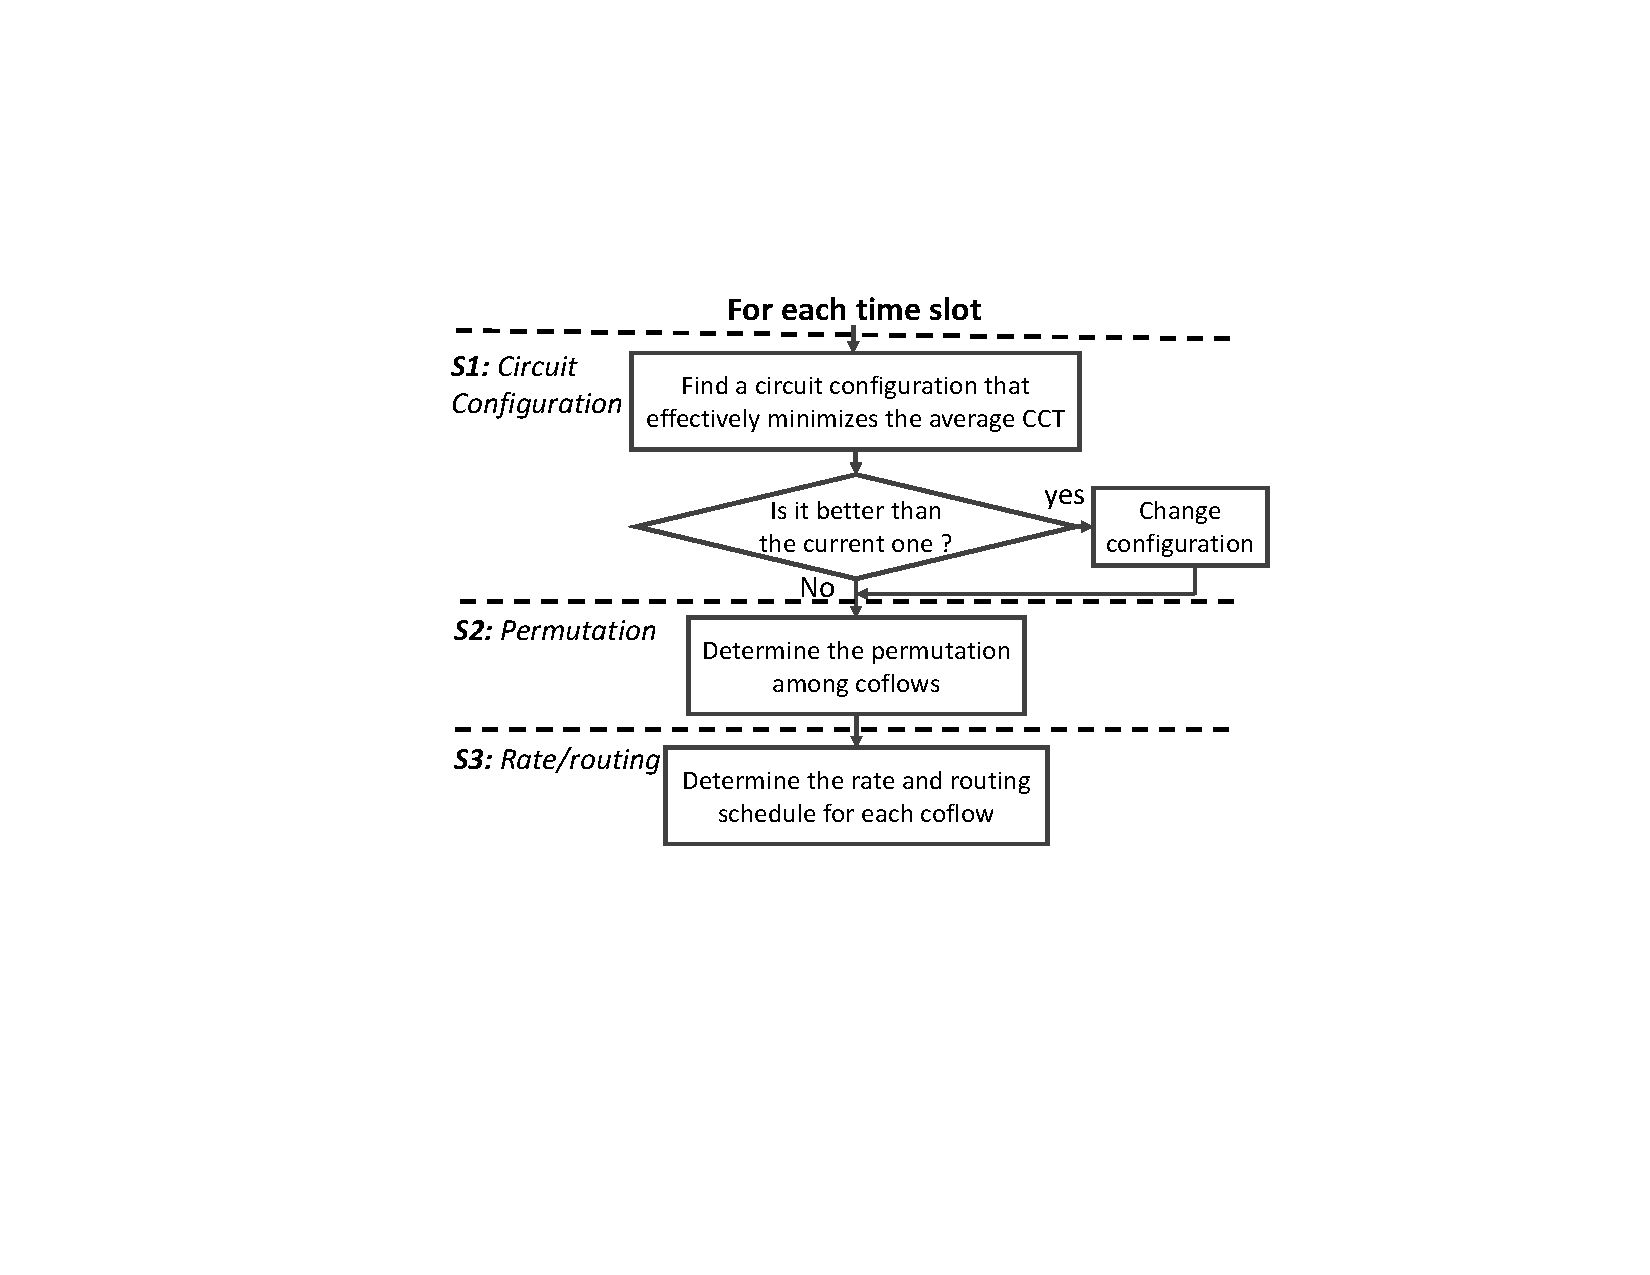
\includegraphics[scale=0.51]{figures/F}%
  \caption{Flow Chart of the Inter-Coflow Scheduling Framework.}
  \label{fig:4}
\end{figure}

Considering the drawbacks of both extremes, we try to reach a sweet point in the middle -- to optimize for the coflows that are likely to be scheduled in the next $T$ timeslots.  The choice of $T$ serves as a flexible knob between the two extremes, and can be effectively tuned via evaluation.
By doing so, we effectively excludes the impact of those far-away coflows, and at the same time reduces the reconfiguration frequency by jointly optimize for high priority coflows. To achieve this, we first
find the $m$ coflows that are likely to be scheduled in the next $T$ timeslots.
We then consider these $m$ coflows as an aggregated coflow $C_{agg}$, and try to find a fixed configuration that well serves their aggregated demand. The problem is then transformed to the joint shaping problem (Problem \ref{problem:3}), and can be solved using Algorithm \ref{ALG-1}.

%It should be positively correlated to the reconfiguration delay $\delta$, and we can effectively tune it via evaluation.
%Note that we
%expose the trade-off with a knob
%reflects a trade-off between long-term and short-term optimization, and it should

Given the new configuration, we must decide whether to reconfigure or not regarding the reconfiguration cost. To do so,
we estimate the CCT for each of the $m$ coflows under the new/old configuration respectively\footnote{The CCTs for the new configuration include an extra reconfiguration delay $\delta$}. Note that the CCT estimation can be described by the coflow shaping problem (Problem \ref{problem:2}).
We then make the decision based on the aggregated CCT of the $m$ coflows.

\parab{Step 2: Permutation}
Given the optimality of the shortest-first policy in
minimizing the average CCT, a natural choice
 would be directly adopt the Smallest-Effective-Bottleneck-First (SEBF) heuristic in Varys \cite{varys}. However, SEBF does not take into account
the underlying circuit configuration when calculating the bottleneck.
Note that this is no longer the case in optical networks, where the bottleneck always depends on the circuit configuration.
%Specially,
%In particular, we have shown that given a coflow demand, the bottleneck always depends on the configuration and the CCT varies greatly under different configurations.
Consequently, we extend the SEBF to CS (configuration-specific)-SEBF by further taking the circuit configuration and routing into consideration. More specifically, given the coflow demand $C$ and the configuration $M$ from Step 1, we calculate the minimum possible CCT $\Gamma$ with coflow reshaping allowed. Note that this is again transformed to the coflow shaping problem (Problem \ref{problem:2}). Coflows are then scheduled in the smallest-$\Gamma$-first order.
%As a result, the CS-SEBF heuristic considers coflow demand, routing and the circuit configuration together,  sorts coflows in the smallest-$\Gamma$-first order.


\parab{Step 3: Routing and Rate Allocation}
Given the circuit configuration (Step 1) and coflow order (Step 2), we can iteratively calculate the routing and rate allocation. More specifically, for each coflow in the smallest-$\Gamma$-first order, we calculate the allocation by solving the coflow shaping problem (Problem \ref{problem:2}) with the current circuit configuration and residual bandwidth. We then update the residual bandwidth according to the allocation, and calculate for the next coflow.


%We leave a in depth evaluation under the general case as future work.





